\section{Theoretical Model}
\label{sec:section2}
\subsection{Setup}\label{sec:section2.1} 
In this section, I establish the theoretical framework for the model developed throughout this paper. Fix a non-atomic continuum of male and female agents and consider the dynamic two-sided market formed by the SBDP, which agents can join to search for potential romantic partners. 
For ease of exposition, I assume that this market is heteronormative such that male agents search exclusively for female agents and vice-versa. 
Time is discrete and indexed by $t=0, 1, 2, ...$ over an infinite horizon. Each period, masses $\lambda_m, \lambda_w>0$ of new men and women enter the platform, where agents are then paired and presented a candidate partner from the opposite side of the market. 

We model agents with heterogeneous preferences (capturing the notion that `beauty lies in the eye of the beholder') and thus, after being paired, each agent observes an \textit{idiosyncratic attractiveness value} $\theta_t \in \Theta := [0,1]$ for their candidate. 
These values are i.i.d according to a pair of absolutely continuous CDF's, $F_m$ and $F_w$, with corresponding PDF's $f_m,f_w$. 
Female agents draw male candidate values from $F_m$ and vice versa but, importantly, the value man $i$ draws for woman $j$ does not necessarily equal the value that $j$ draws for $i$ and, for simplicity, these are modelled as independent from one another.

After observing their candidate's attractiveness, agents then choose to swipe left (dislike) or right (like) on them, yielding an action space $\mathcal{A}=\{ 1, 0\}$, where $a_t=1$ indicates a right-swipe. 
If either agent swipes left, then they both receive a payoff of zero; however, if both agents swipe right, they are said to have \textit{matched} and both receive a matching payoff $u(\theta_t)$, where $u(\cdot)$ is a continuous, strictly increasing function that satisfies $u(0) = 0$. 
This last property stems from the fact that, in most SBDPs, users are allowed to unmatch with each other, and therefore matching with even the least attractive individual on the other side of the market is weakly preferred to not matching. 

After payoffs have been received, agents are paired with different candidates and the stage interaction is repeated. Given the continuum of agents, I assume that interactions take place \textit{anonymously} in the style of \cite{jovanovic1988anonymous}. Furthermore, to the agents' knowledge, pairings are determined in an unknown manner (since SBDPs are generally secretive regarding the algorithms they use), effectively making their problem one of uniform random search.

\begin{figure}[ht]
    \centering 
    \caption{Sequence of events within each time period}
    \vspace{20pt} 
        \begin{tikzpicture}
            % draw horizontal line   
        \draw[thick, -Triangle] (0,0) -- (\ImageWidth,0); %node[font=\scriptsize,below left=3pt and -8pt]{$t+1$};

        % draw vertical lines
        \foreach \x in {1,2,...,6}
        \draw (\x*2 cm,4pt) -- (\x*2 cm,-4pt);

        \foreach \x/\descr in {2/t, 4/\text{Arrivals}, 6/\text{Pairings}, 8/\text{Game Play}, 10/\text{Departures}, 12/t+1}
        \node[font=\scriptsize, text height=1.75ex,
        text depth=.5ex] at (\x,-.3) {$\descr$};  
    \end{tikzpicture}
    \label{fig:timeline}
\end{figure}

Since swiping right in the above stage game is weakly dominant for all agents, one would not expect the repeated interaction to be massively revealing of real-life preferences, where initiating a romanic encounter is often perceived by humans as a costly endeavour \citep{dawkins2017selfish}. This becomes problematic since the main selling point of SBDPs is a reduction in searching costs for individuals seeking romantic encounters, and this is only accomplished if matches have a high likelihood of resulting in real-life romantic attraction. Because of this, SBDPs like Tinder place a cap on the total number of right swipes for each user, thus enabling this as a form of costly signalling. I refer to the total number of right-swipes a user has left as its \textit{budget}, $b$, which evolves dynamically according to the law of motion: 
\begin{equation*} 
  b_{t+1}= b_{t} - a_t
\end{equation*}

The budget sets for men and women are thus defined by $\mathcal{B}_{s}=\{b \in \mathbb{Z} : 1\leq b \leq B_s\}$, for each sex $s=m,w$, with budget caps $B_m$ and $B_w$ determined exogenously. Importantly, agents depart from the platform in one of two ways: they can leave \textit{endogenously}, if they expend their swiping budget, or \textit{exogenously} with probability $(1-\delta)$ in each time period. This admits to the interpretation of a geometrically distributed lifetime, such that agents discount future payments by a factor of $\delta\in(0,1)$. 

One final remark for this setup is that, in a continuum market with anonymous interactions, the mean-field assumption established in \autoref{sec:section2.3} effectively restricts focus onto the set of (pure) symmetric stationary strategies. This is argued in more detail in the following sections but, for now, denote these strategies by functions $\mu: \Theta \times\mathcal{B}_m\rightarrow \mathcal{A}$ for men and $\omega:\Theta \times\mathcal{B}_w\rightarrow \mathcal{A}$ for women.

\subsection{The Dating Market}\label{sec:section2.2}
With the above framework in place, I now outline the platform state variables that make up the SBDP market. 
Let $N_{mt}(b), N_{wt}(b)$ denote the mass of male and female agents (respectively) with a budget of $b\in\mathcal{B}$ in a given time period $t$. 
%Additionally, with a slight abuse of notation, let $N_{mt}, N_{wt}$ denote the overall mass of male and female agents (respectively) in the platform, i.e. $\sum_{b\in\mathcal{B}_m}N_{mt}(b)$ and $\sum_{b\in\mathcal{B}_w}N_{wt}(b)$.
Since gender imbalances can leave some agents in the long side of the market unpaired, a pairings process must also be determined. 
Given the automated nature of SBDPs, I assume an efficient matching technology and model pairings as a Bernoulli process parametrised by market tightness; thus, the probability of being paired with a candidate is defined for both sides as:  
\begin{equation*}
    \tau_{mt}:=\min \left\{\frac{\sum_{b\in\mathcal{B}_w}N_{wt}(b)}{\sum_{b\in\mathcal{B}_m}N_{mt}(b)} , 1 \right\}, 
    \quad \tau_{wt}:= \left(\frac{\sum_{b\in\mathcal{B}_m}N_{mt}(b)}{\sum_{b\in\mathcal{B}_w}N_{wt}(b)} \right) \tau_{mt} 
\end{equation*}

From the above, the platform state in time period $t$ can be defined as $\Psi_t=(N_{mt},N_{wt})$. 
For most of this paper, I focus on characterising user behaviour and its resulting implications in a stationary setting (which is denoted by omitted time subscripts), although some discussion of coupled strategy and market dynamics is provided in \autoref{sec:section4}. 
As a necessary requirement, the market steady state $\Psi_t=\Psi_{t+1}=...=\Psi$ must satisfy the balanced flow conditions \footnote{Formally, these conditions rely on the exact law of large numbers, which was rigorously developed in discrete-time settings by \cite{duffie2018dynamic}, but a technical discussion of this lies outside the scope of this paper.} for our continuum model; these are presented below for the female agents, but they apply analogously to the male side of the market. 
Firstly, the entry flow of agents into the platform must equal the departure flow: 
\begin{equation}\label{eq:ss1} 
    \lambda_w\;=\; \underbrace{ (1-\delta)\sum_{b\in\mathcal{B}_w}N_{w}(b)}_{\text{Exogenous Outflow}} \;+\; \underbrace{N_w(1) \delta \tau_w\int_{\Theta}\omega(\theta,1)\,dF_{m}(\theta)}_{\text{Endogenous Outflow}} 
\end{equation} 

Secondly, for both sides, the flow of agents into any particular budget level must equal the outflow of agents from that same level. Thus, for all $b\in\mathcal{B}_w$: 
\begin{equation}\label{eq:ss2} 
    \underbrace{N_w(b+1) \delta \tau_w \int_{\Theta} \omega(\theta,b+1)\,dF_{m}(\theta)}_{\text{Inflow into $b$}} \;=\; \underbrace{N_w(b) \Big( (1-\delta) \;+\; \delta \tau_w\int_{\Theta} \omega(\theta,b)\,dF_{m}(\theta)\Big)}_{\text{Outflow from $b$}}
\end{equation}

Finally, the entry flow of agents into the platform must equal the outflow from the top budget level, hence: 
\begin{equation}\label{eq:ss3} 
    \lambda_w \;=\; \underbrace{N_w(B_w) \Big( (1-\delta) \;+\; \delta \tau_w \int_{\Theta} \omega(\theta,B_w)\,dF_{m}(\theta) \Big)}_{\text{Outflow from $B_w$}}
\end{equation} 

Importantly, the above conditions take the strategy profile $(\mu,\omega)$ as exogenously fixed. Over the next section, these are endogenously derived by characterising the agents' best-responses in an SDBP setting, which themselves depend on the market steady state $\Psi$.

\subsection{The Search Problem}\label{sec:section2.3}
With the model framework outlined above, I now present the decision problem faced by female agents in the market given some platform steady state $\Psi$, with analogous results and implications for the male side. 
Consider now a woman $i$ who is paired with a man $j$ in the platform. Since $j$'s swiping behaviour will depend on his own budget, which is unknown to woman $i$, then (under strict rationality) she would have to compute her expected payoff conditional on her beliefs for the market history.

This behaviour is both unreasonable and intractable in an SBDP setting, as explained in \autoref{sec:section1.1}; instead, given a stationary platform and a continuum of anonymous agents, it is reasonable to conjecture that the average swiping rate for men, $\overline\mu$, is also stationary, and that any individual agent's actions have a negligible effect on the platform state dynamics\footnote{I also assume that $\overline\mu>0$ to prune out degenerate equilibria where one side never swipes right.}.
As such, the expected ex-interim payoff for woman $i$ is the following:
\begin{equation*}
    \begin{aligned}
        U(\theta, a)&= \,\overline{\mu} a u(\theta)%, \\[8pt] \quad \text{where}\quad \overline{\mu} &= \sum_{b\in \mathcal{B}_m}\int_{\Theta}\frac{{N}_m(b)}{N_m}  \, \mu(\theta',b)\,dF_w(\theta')
    \end{aligned} 
\end{equation*} 

The above imposes a mean-field assumption, such that woman $i$ accounts for $j$'s behaviour only through $\overline\mu$ conditional on the platform state $\Psi$.
This modelling choice, which has been employed by \cite{immorlica2021designing} and \cite{iyer2014mean} among others, simplifies the full dynamic game by collapsing it onto a pair of Markov Decision Processes (MDPs), one for each side of the market, such that strategy $\omega$ is a best-response for women iff it is an optimal policy for the corresponding MDP. 
Additionally, this also condenses $i$'s state of payoff-dependent variables to include only the value $\theta$ that she observes for $j$ and her own budget $b$. 
Therefore, since all agents in the same side solve the same MDP, which depends only on their individual state, this effectively justifies the restricted focus on symmetric stationary strategies, as established in \autoref{sec:section2.1}.

Let the unrealized jump times of the pairing process for woman $i$ be indexed by $k$. 
Given that, at the time of pairing, this women has a budget of $b$ right swipes left, she then solves the constrained MDP presented below, captured by the value function $V_w(\theta,b)$: 
\begin{equation*}
    \begin{aligned} 
        V_w(\theta,b)=\max_{\{a_k\}^\infty_{k=0}} \quad & \mathbb{E}_{\theta}\left[\sum^\infty_{k=0} \delta^{k} U(\theta_k, a_k) \;|\; \theta_0=\theta, b_0=b\right]\\ 
        \textrm{s.t.} \quad & b_{k+1} = b_k - a_k \\
        & b_k\in \mathcal{B}_w \cup \{0\},\\
        & a_k\in \mathcal{A}  
    \end{aligned}
\end{equation*}

Importantly, the first two constraints, along with the exogenous departure process, make this problem non-trivial: by limiting woman $i$'s right-swiping budget, the platform imposes an opportunity cost for swiping right on $j$ and foregoing potential future matches with more attractive men, whilst the exogenous departure process removes the possibility of simply waiting around to swipe right on the top-$B_w$ most attractive men in the platform. 
By standard dynamic programming arguments, this problem can be captured by two Bellman equations; one for when $j$ is paired and another for when she isn't: 
\begin{align}
    \begin{split} 
        V^{P}_w(\theta,b) &=\max \Big\{ \, \overline{\mu}\, u(\theta) \;+\; \delta \tau_w \,\mathbb{E}_\theta \Big[V^P_w(\theta', b-1)\Big] \;+\; \delta (1-\tau_w)V^{NP}_w(b-1) \, ,\\[6pt]
        & \quad\quad\quad\quad\;\delta \tau_w \, \mathbb{E}_\theta\Big[ V^P_w(\theta', b) \Big] \;+\; \delta (1-\tau_w) V^{NP}_w(b) \, \Big\}
    \end{split}\\[10pt]
    \begin{split}
        V^{NP}_w(b) &= {}\delta \tau_w \,\mathbb{E}_\theta \Big[ V^P_w(\theta', b)\Big] \,+\, \delta (1-\tau_w) V^{NP}_w(b)
    \end{split} 
\end{align} 

With some straightforward algebra, the above two equations can be merged into the full Bellman equation below. Note that the swiping budget constraint from the above MDP imposes the boundary condition $V_w(\theta, 0)=0$ for all $\theta \in \Theta$, since agents who expend their budget must leave the platform and can't accumulate any additional payoffs: 
\begin{equation}\label{eq:full bellman}
    \begin{aligned} 
        V_w(\theta,b) \;=\;&\max\left\{\,\overline{\mu} \, u(\theta) +\alpha \,\mathbb{E}_\theta \Big[V_w(\theta', b-1)\Big]\,,\; \alpha\,\mathbb{E}_\theta \Big[ V_w(\theta', b)\Big]\,\right\}
    \end{aligned}
\end{equation}

Here, $\alpha$ is the effective discount rate accounting for the exogenous possibilities of both departures and pairings, defined as:  
\begin{equation*}
\alpha:=\frac{\delta \tau_w}{1-\delta(1-\tau_w)}.
\end{equation*}

Upon inspection, it is clear that the value function is of a piecewise nature over $\Theta$. This is formally stated below (with the corresponding derivation included in \autoref{appx: b}): 
\begin{proposition}\label{prop:piecewiseV}
Fix some $b\in\mathcal{B}_w$. Then there exists some unique reservation value $\widetilde{\omega}_b\in \Theta$ such that $V_w(\theta,b)$ admits the following piecewise form over $\Theta$:  
\begin{equation*}
    \begin{split}
        V_w(\theta,b)=\begin{cases}
            \overline\mu u(\theta) +\alpha \,\mathbb{E}_{\theta}\Big[V_w(\theta', b-1)\Big],& \theta \geq \widetilde \omega_b \\[10pt]
            \alpha \,\mathbb{E}_{\theta}\Big[V_w(\theta', b)\Big],& \theta\leq\widetilde \omega_b
        \end{cases}\\[8pt]  
    \end{split}
\end{equation*} 
\end{proposition}  

In the result above, all reservation values $\{\widetilde\omega\}_{b\in \mathcal{B}_w}$ are such that woman $i$ is indifferent between swiping left or right. Therefore, an optimal policy for woman $i$'s MDP involves swiping right for partners who exceed the reservation value for her current budget:  
\begin{corollary}\label{cor:optpolicy}
    The following threshold policy $\widetilde\omega$, parametrised by $\{\widetilde\omega\}_{b\in \mathcal{B}_w}$, attains $V_w(\theta,b)$:
    \begin{equation*}
        \begin{split}
            \widetilde\omega(\theta,b)&=\begin{cases}
                \text{Swipe Right},\quad \theta\geq \widetilde{\omega}_b \\ 
                \text{Swipe Left}, \quad\theta< \widetilde\omega _b  
            \end{cases}   
        \end{split}
    \end{equation*} 
\end{corollary} 

Using both of these results, I now derive the following explicit characterisation for reservation values $\{\widetilde\omega_b\}_{b\in \mathcal{B}_w}$ (with a corresponding proof included in \autoref{appx: b}). 
\begin{proposition}\label{prop:recurrence relation}
The set of reservation values for women, $\{\widetilde\omega_b\}_{b\in \mathcal{B}_w}$, uniquely satisfies the recurrence relation and initial condition below, over the budget set $\mathcal{B}_w$: 
\begin{equation}\label{eq:recurrence relation}
    \begin{aligned}
        u(\widetilde \omega_b) \;=\; \alpha u(\widetilde \omega_b) F_m(\widetilde \omega_b) \;+\; \alpha u(\widetilde \omega_{b-1}) \Big[1- F_m(\widetilde \omega_{b-1})\Big] \;+\; \int^{\widetilde \omega_{b-1}}_{\widetilde \omega_b} \alpha u(\theta')\,dF_m(\theta')
    \end{aligned} 
\end{equation}  
\begin{equation}\label{eq:initial condition}
    u(\widetilde\omega_1) \;=\; \alpha u(\widetilde\omega_1)F_m(\widetilde\omega_1) \;+\; \alpha \int^1_{\widetilde\omega_1}u(\theta')\,dF_m(\theta')
\end{equation}
\end{proposition}  

This explicit characterisation allows for an improved computation of $\{\widetilde\omega_b\}_{b\in \mathcal{B}_w}$ over traditional numerical methods such as value iteration \citep{bellman2015applied}, which has a runtime complexity of $\mathcal{O}(|\mathcal{B}_w\times\Theta|^2|\mathcal{A}|)$ and can become expensive for large budget sets or fine discretisations of $\Theta$. Using the recurrence relation in \autoref{prop:recurrence relation}, the optimal policy was computed for an arbitrary set of exogenous parameters, with results in \autoref{fig:swiping-rule} showing a clear cut-off rule for swiping right. 
These cut-off values are decreasing in the agent's budget, which captures the notion that an agent's current swipe is more valuable than all preceding ones given the increasing opportunity cost.

\begin{figure}[ht]
    \centering
    \caption{The Optimal Swiping Rule}
    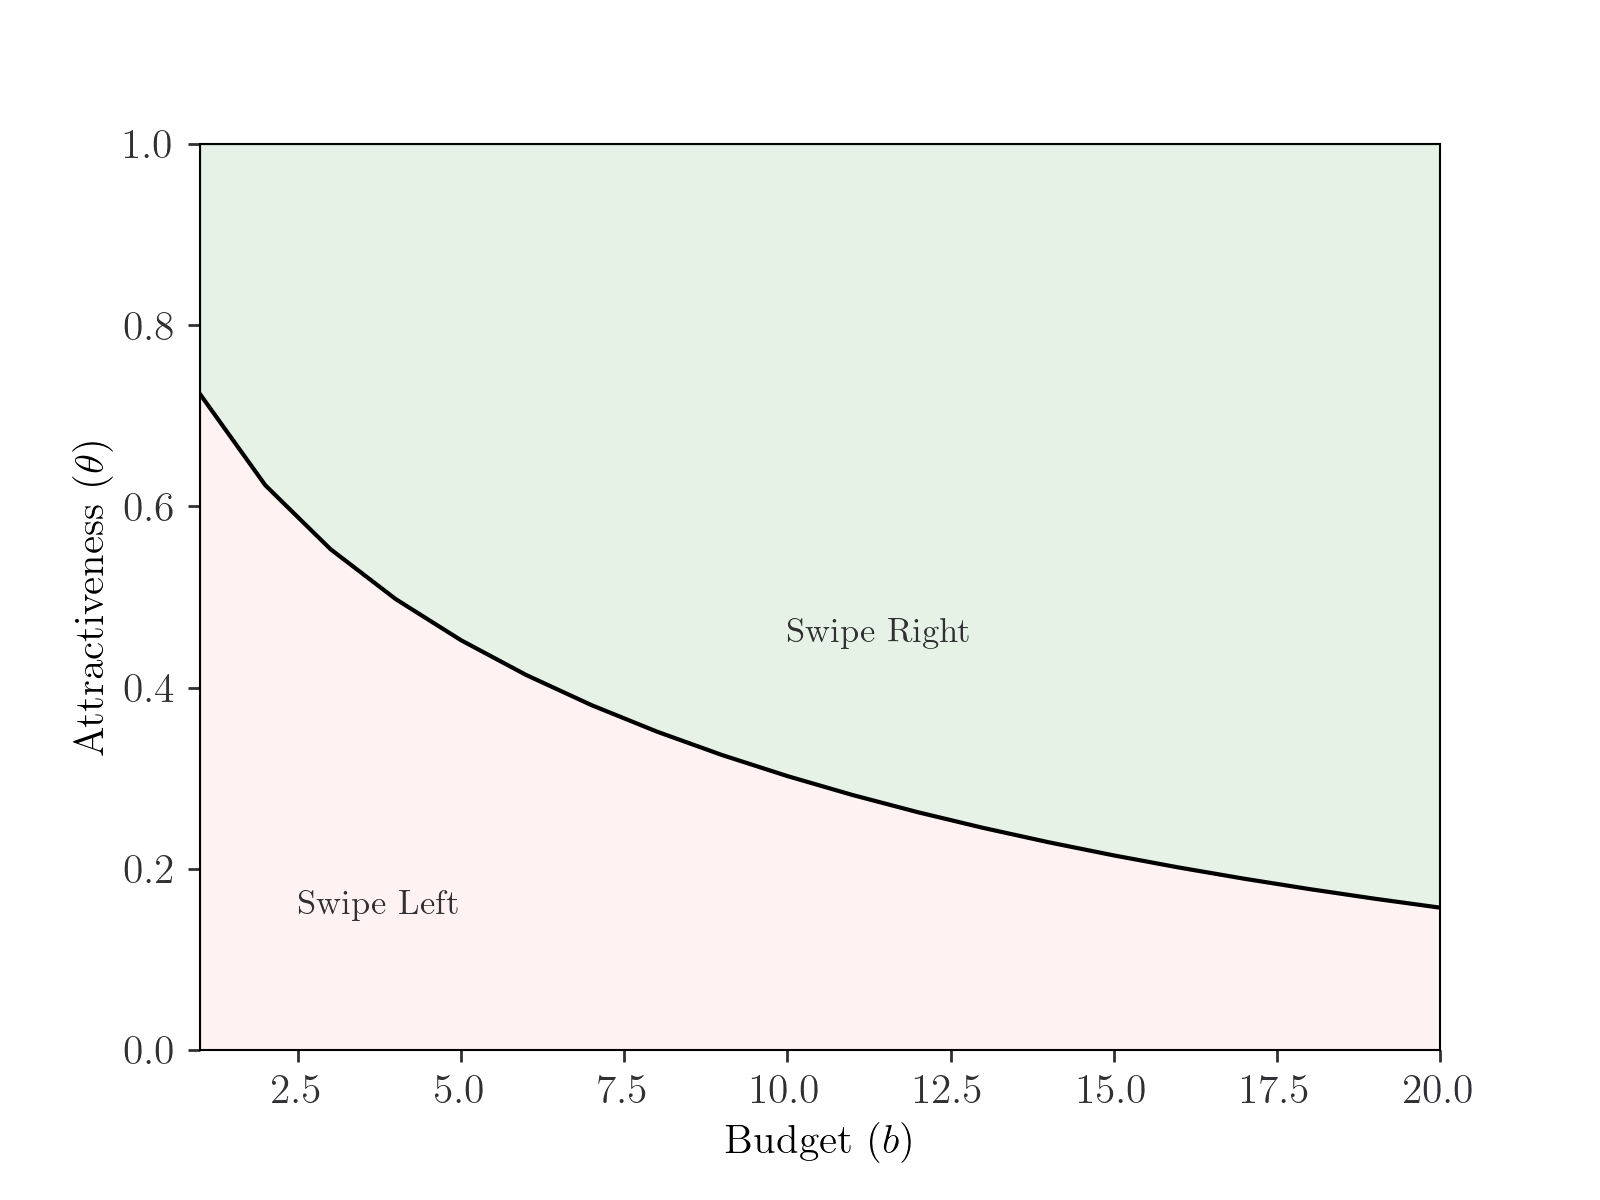
\includegraphics{swiping-rule.png}
    \label{fig:swiping-rule} 
\end{figure} 